\documentclass{main.tex}[subfiles]
\begin{document}
\newpage
\nonumsection{Приложение 1. Дополнительные иллюстрации}

%\begin{figure}[H]
%    \centering
%    \includegraphics[width=\myPictWidth]{ovodov_forum}
%    \caption{И.Г. Оводов представляет проект распознавания шрифта Брайля по фотографии на форуме <<Сильные идеи для нового времени>>. Кадр телеканала <<Россия 24>> \protect\footnotemark}
%    \label{fig:ovodov_forum}
%\end{figure}
%
%\footnotetext{\href{https://youtu.be/SVocn-tnjz8?t=5427}{Форум АСИ "Сильные идеи для нового времени". Полная версия (YouTube)}}

\begin{figure}[H]
    \centering
    \begin{subfigure}{.5\textwidth}
        \centering
        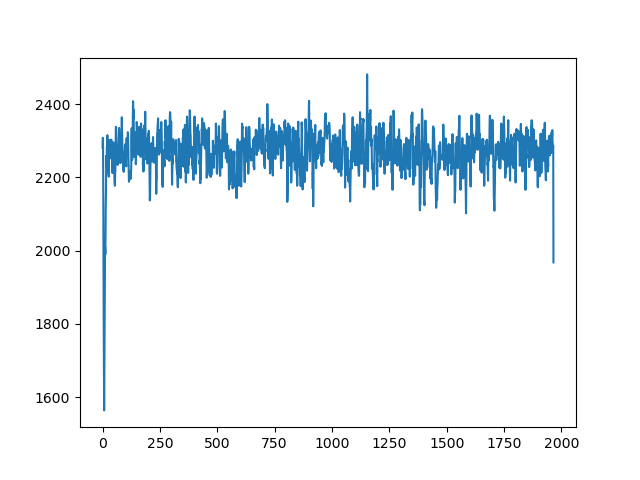
\includegraphics[width=\myPictWidth]{test_find_regions/find_regions_k2}
        \caption{$ k = 2 $}
        % TODO \label{fig:}
    \end{subfigure}%
    \begin{subfigure}{.5\textwidth}
        \centering
        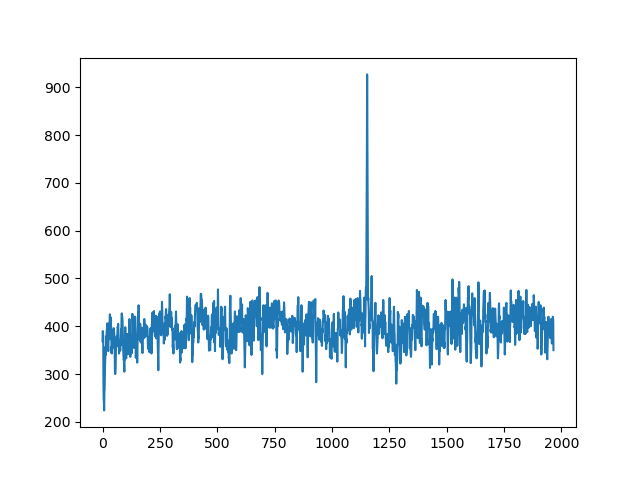
\includegraphics[width=\myPictWidth]{test_find_regions/find_regions_k4}
        \caption{$ k = 4 $}
        % TODO \label{fig:}
    \end{subfigure}

    \begin{subfigure}{.5\textwidth}
        \centering
        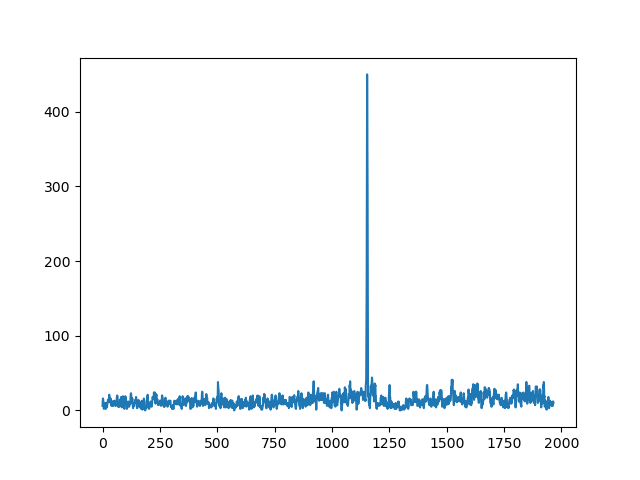
\includegraphics[width=\myPictWidth]{test_find_regions/find_regions_k8}
        \caption{$ k = 8 $}
        % TODO \label{fig:}
    \end{subfigure}%
    \begin{subfigure}{.5\textwidth}
        \centering
        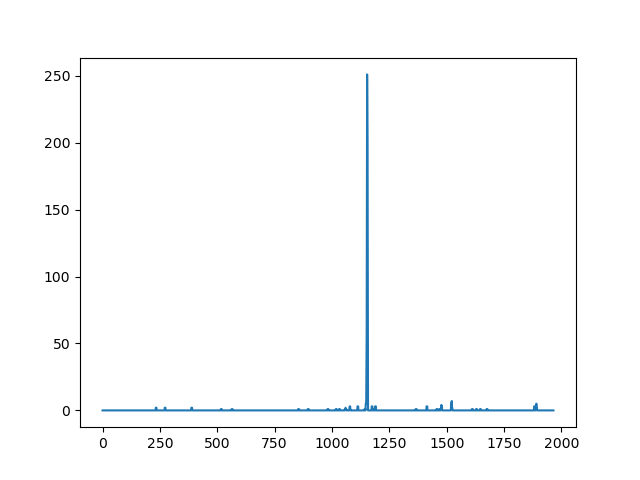
\includegraphics[width=\myPictWidth]{test_find_regions/find_regions_k15}
        \caption{$ k = 15 $}
        % TODO \label{fig:}
    \end{subfigure}
    \caption{Зависимость числа k-грам, найденных в регионе исходного текста, от позиции региона относительно начала текста}
    \label{fig:find_k}
\end{figure}

\begin{figure}[H]
    \centering
    \begin{subfigure}{.5\textwidth}
        \centering
        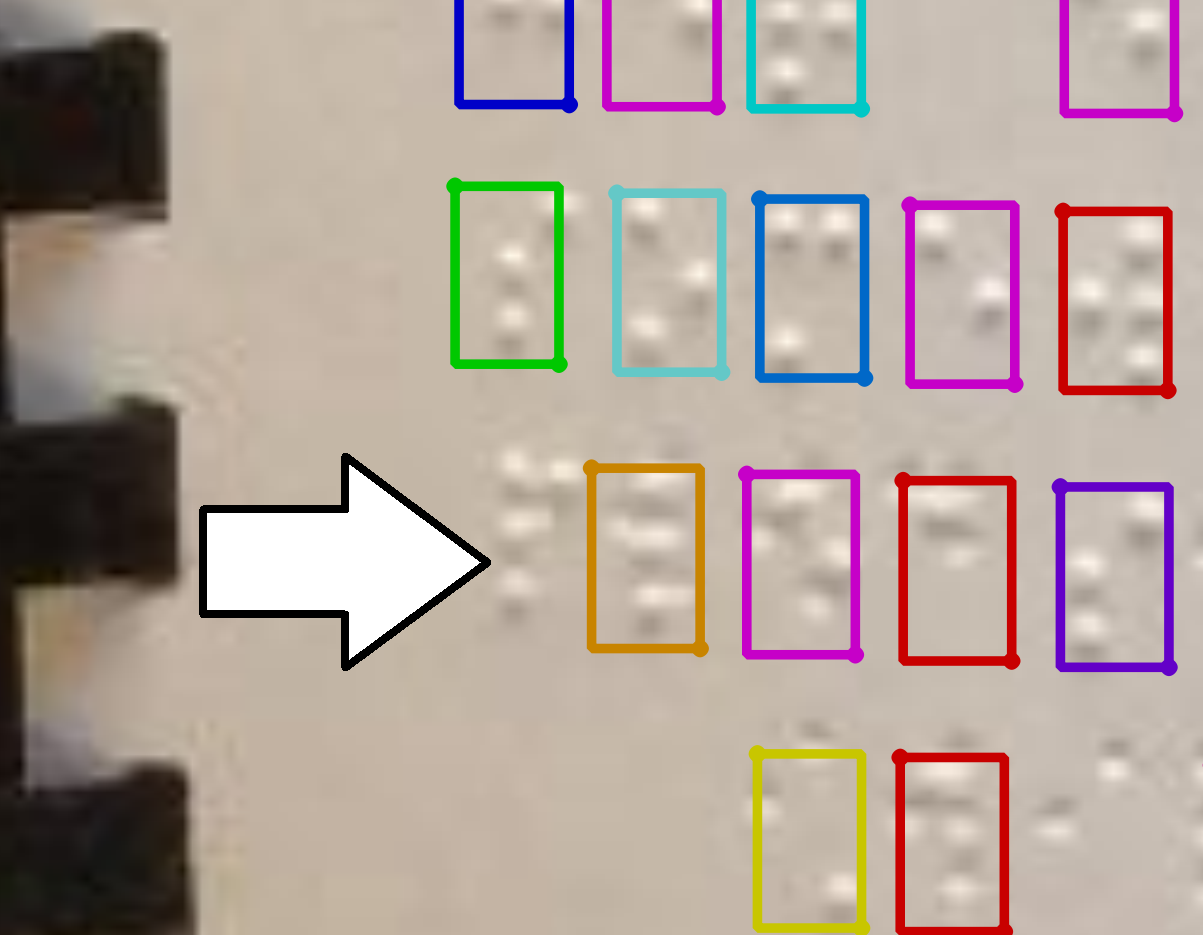
\includegraphics[width=.95\myPictWidth]{recogn_mistakes/deletion}
        \caption{Выпадение символа}
        \label{fig:recogn_mistakes:del}
    \end{subfigure}%
    \begin{subfigure}{.5\textwidth}
        \centering
        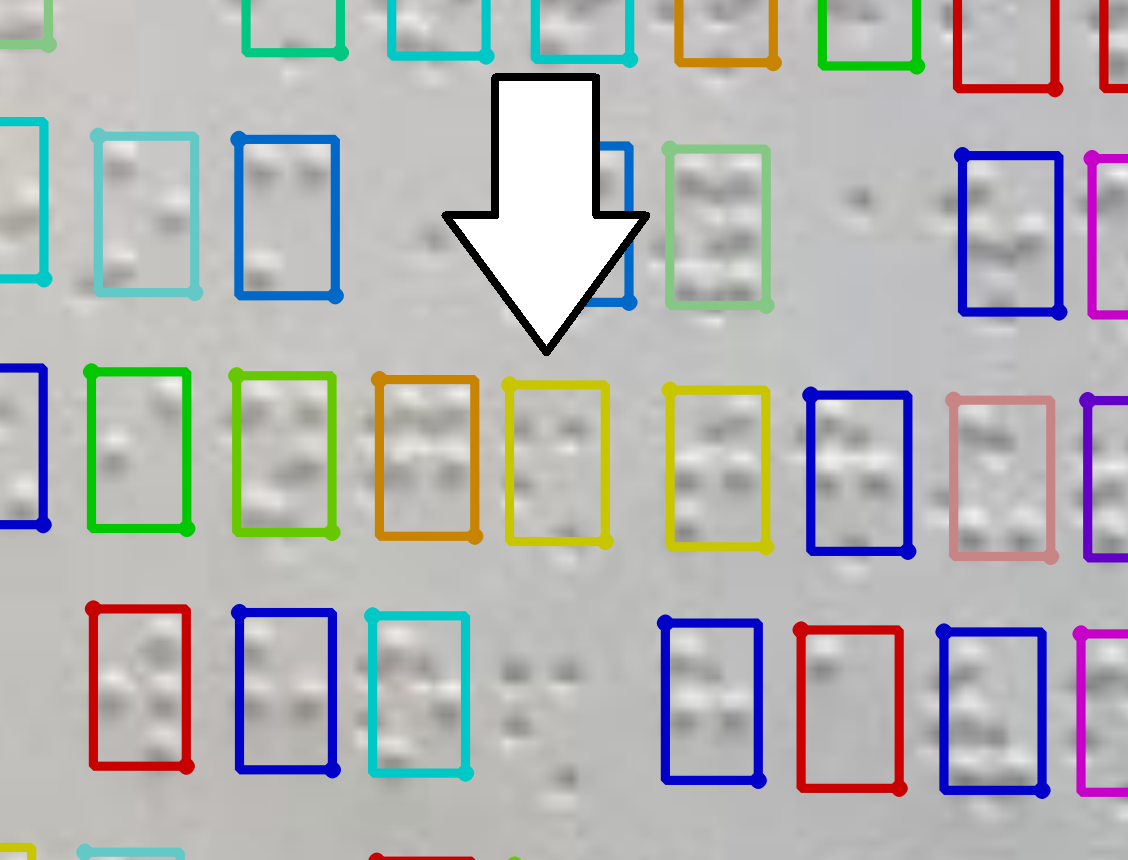
\includegraphics[width=.95\myPictWidth]{recogn_mistakes/insertion}
        \caption{Вставка символа}
        \label{fig:recogn_mistakes:ins}
    \end{subfigure}

    \begin{subfigure}{.5\textwidth}
        \centering
        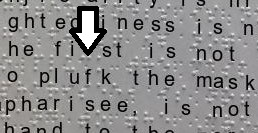
\includegraphics[width=.95\myPictWidth]{recogn_mistakes/mismatch}
        \caption{Неверно распознан символ}
        \label{fig:recogn_mistakes:mismatch}
    \end{subfigure}%
    \begin{subfigure}{.5\textwidth}
        \centering
        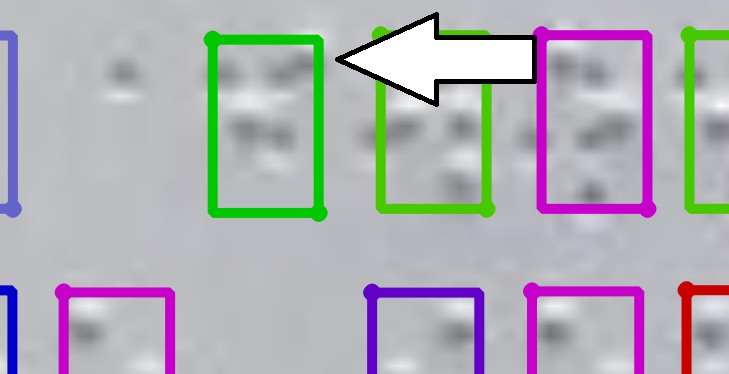
\includegraphics[width=.95\myPictWidth]{recogn_mistakes/misplaced_label}
        \caption{Неверно обозначены границы объекта}
        \label{fig:recogn_mistakes:misplaced_label}
    \end{subfigure}
    \caption{Разновидности ошибок распознавания}
    \label{fig:recogn_mistakes}
\end{figure}

\newpage
\nonumsection{Приложение 2. Исходный код программ}
Ниже приведён исходный код программы, реализующей модифицированный алгоритм Нидлмана-Вунша. % TODO ссылка на номер алгоритма
Этот код, а также программы, осуществляющие поиск регионов интереса, вспомогательные манипуляции с изображением (обрезка, переименование...) и текстом (замена символов, подсчёт статистик...) доступны в репозитории\footnote{\href{https://github.com/braille-systems/brl_data_tools}{github.com/braille-systems/brl\_data\_tools}}.
Там же можно найти инструкцию по установке и запуску, а также сслыки для загрузки файлов с исходными данными (файл \texttt{README.md}).

\lstinputlisting{../../scripts/needleman_wunsch.py}
\end{document}